\section{Introduction}

In a true many-body electronic wave function, the motions of electrons are dynamically correlated across the entire range of inter-electronic distances.
A large part of this correlation is efficiently captured by various approximations to the Kohn--Sham density-functional theory (KS-DFT), which made it a basic tool in computational chemistry and condensed-matter physics.
But the standard density functionals are semi-local in space, resulting in electron correlation that decays exponentially with distance and electrons that are essentially uncorrelated at long range.
This often leads to severe underestimation of van der Waals (vdW) dispersion interactions, which are mostly caused by long-range electron correlation, and which strongly contribute to properties of most biological and modern synthetic materials.
As a result of this deficiency, many models accounting specifically for the long-range correlation were developed~\cite{DionPRL04,VydrovJCP10a,BeckeJCP07,TkatchenkoPRL09,GrimmeJCP10,AmbrosettiJCP14} and combined with semi-local (or hybrid) density-functional calculations.
This range separation of electron correlation into two separate models can be in principle done formally~\cite{HermannCR17}, but insufficient knowledge about the (differing) ranges of semi-local functionals prevents it in practice, leading to various semi-empirical approaches.

The SCAN functional is a recent first-principles semi-local functional~\cite{SunPRL15} with great performance across a broad range of systems in chemistry and physics, in many cases reaching the accuracy of hybrid functionals at a fraction of their cost~\cite{SunNC16}.
Being semi-local, however, it still does not describe long-range electron correlation, and hence vdW interactions.
The many-body dispersion (MBD) method is a general model of long-range electron correlation~\cite{TkatchenkoPRL12,AmbrosettiJCP14} that can be combined with any short-range correlation method, such as semi-local DFT or the density-functional tight-binding method.
The crossover regime, where a short-range description blends with the long-range MBD description, is controlled with a single range-separation parameter within the MBD model.
When trying to adjust this parameter for the SCAN functional---essentially estimating the correlation range of SCAN for vdW interactions---we observed that the optimal value depends substantially on the choice of the studied systems and the choice of the optimized quantity.
Since this is not the case for other density functionals such as PBE, we set out to study in general the range of electron correlation as described by different density functionals in vdW-bound systems.

\section{Background}

systems: S66~\cite{RezacJCTC11}, X23~\cite{ReillyJCP13}, S12L~\cite{RisthausJCTC13}

vdW methods: D3~\cite{GrimmeJCP10}, VV10~\cite{VydrovJCP10a}, MBD

functionals: LDA~\cite{DiracMPCPS30,PerdewPRB92}, PBE~\cite{PerdewPRL96}, PBE0~\cite{AdamoJCP99}, B3LYP~\cite{BeckeJCP93}, SCAN, M06~\cite{ZhaoTCA08}, TPSS~\cite{TaoPRL03}.

\section{Calculations}

Several aspects of the ``tail'' behaviour of semi-local density functionals in vdW systems are known, mostly from observations made on particular systems.
The Hartree--Fock model separates electron correlation into the exchange and ``pure'' correlation parts, the second of which is exclusively responsible for vdW attraction.
This does not translate well into exchange and correlation as approximated by semi-local density functionals in DFT, where the exchange part often contributes much more than the correlation part to the binding at equilibrium distances.
This behaviour is caused by the implicit cancellation of errors between the two parts, and is reflected by the fact that most of the literature on this topic is concerned with exchange, not correlation functionals.
The search for semi-local functionals with the appropriate range of correlation have been done mostly in the context of the vdW-DF non-local functional~\cite{CooperPRB10,PernalPRL09,KlimesJPCM10,KlimesPRB11,HamadaPRB14,WellendorffPRB12,BerlandPRB14}, a long-range correlation method which is not easily adapted to different density functionals~\cite{DionPRL04,LeePRB10}.
Still, a more common approach is to consider the range of a semi-local functional fixed, and tune the long-range correlation model for that range, usually by adjusting a small number of parameters (often one).
In both approaches, the resulting DFT+vdW methods are mostly designed and assessed numerically, by evaluating them on some benchmark systems where accurate binding energies are known from high-level correlation methods or experiment.
In this work, we resort to the same technique, but considerably expand the number of system types, functionals, and vdW methods contained within a single study, which gives us a novel insight into the behaviour of different functionals.

\section{Background}

In a general beyond-LDA exchange functional, the exchange energy density of a uniform electron gas, $\varepsilon^\text{unif}_\text x(n)=-3k_\mathrm F(n)/4\pi$, $k_\text F(n)=(3\pi^2n)^{1/3}$, is multiplied with the so-called enhancement factor, $F_\text x[n](\mathbf r)$,

$$
E_\text x[n]=\int\mathrm d\mathbf rn(\mathbf r)\varepsilon^\text{unif}_\text x(n(\mathbf r))F_\text x[n](\mathbf r)
$$

In LDA, $F^\text{LDA}_\text x(\mathbf r)=1$.
In GGA, $F_\text x[n](\mathbf r)=F^\text{GGA}_\text x(s(\mathbf r))$, where $s[n]=\lvert\boldsymbol\nabla n\rvert/2k_\text F(n)n$ is the (dimensionless) reduced density gradient.
In meta-GGA, higher derivatives of the electron density are used to construct $F_\text x$, such as the Laplacian, as well as the KS kinetic energy density, $\tau[n]=\sum_i^\text{occ}\lvert\boldsymbol\nabla\phi_i\rvert^2/2$, where $\phi_i$ are the KS orbitals.
In the SCAN functional specifically, the dependence on the kinetic energy density is introduced via the local density parameter $\alpha[n](\mathbf r)$,
$$
\alpha=(\tau-\tau^\text W)/\tau^\text{unif}\geq0
$$
where $\tau^\text W[n]=\lvert\boldsymbol\nabla n\rvert^2/8n$ is the von Weizsäcker kinetic functional, exact for single-orbital electron densities, and $\tau^\text{unif}(n)=3k_\text F(n)^2n/10$ is the Thomas--Fermi kinetic functional, exact for the uniform electron gas.
The motivation for the use of $\alpha$ is that $\alpha\approx0$ where a single orbital dominates the electron density, $\alpha\approx1$ in the slowly varying (metallic) electron densities, and $\alpha\gg0$ where two closed-shell densities overlap, which is characteristic of vdW interactions.
So in SCAN, $F_\text x[n](\mathbf r)=F_\text x^\text{SCAN}(s(\mathbf r), \alpha(\mathbf r))$.
This richer form enables it to satisfy a wider range of exact constraints, norms, and limits compared to GGA functionals.

We use three vdW models to characterize the correlation-range behaviour of the XC functionals: many-body dispersion (MBD), D3 of Grimme, and the Vydrov--Van Voorhis 2010 non-local functional (VV10).
Because the correlation range differs between XC functionals, and in any case is explicitly unknown, all these vdW models have parameters that control their own correlation range, and enables them to be adjusted for different XC functionals.
Here, we review only those aspects of these vdW models directly related to these correlation-range parameters, while we refer the reader to the original references for full descriptions.
In MBD, the electronic Coulomb potential, $v(r)$, (precisely, its dipole approximation, $\mathbf T(\mathbf r-\mathbf r')=\boldsymbol\nabla_\mathbf r\boldsymbol\nabla_\mathbf r'v(\lvert\mathbf r-\mathbf r'\rvert)$) is explicitly damped at short distances with a logistic function,
$$
  \mathbf T^\text{MBD}(\mathbf R_i-\mathbf R_j)=\frac{\mathbf T(\mathbf R_i-\mathbf R_j)}{1+\exp\left(-6\left(\frac{\lvert\mathbf R_i-\mathbf R_j\rvert}{\beta\big(R_i^\text{vdW}+R_j^\text{vdW}\big )}-1\right)\!\!\right)}
$$
where $R_i^\text{vdW}$ is a vdW radius of the $i$-th atom, and $\beta$ is the single range-separation parameter.
The damped dipole potential is equal to a half of the bare potential at the distance that is a $\beta$-fraction of the sum of vdW radii of two atoms.
In D3, being a second-order approximation to the full many-body correlation problem, the radially-averaged square of the dipole--dipole and dipole--quadrupole potentials are used, $\langle\mathbf T_{pp}^2\rangle=6R^{-6}$, $\langle\mathbf T{pQ}^2\rangle=8R^{-8}$, which are then damped explicitly at short distances.
Several different damping functions have been suggested, but we consider only the Becke--Johnson (BJ) damping, being most popular and also mostly different from the MBD damping function,
$$
  f_n^\text{BJ}(R_{ij})R_{ij}^{-n}=\frac{R_{ij}^{-n}}{1+\left(\frac{\alpha_1(R^0_i+R^0_j)+\alpha_2}{R_{ij}}\right)^n}
$$
where $R^0_i$ is a vdW-like radius of the $i$-th atom, and $\alpha_1$, $\alpha_2$ are two range-separation parameters.
The D3 energy is then obtained as
$$
E^\text{D3}_\text{vdW}=-\frac12\sum_{ij}C_{6,ij}f_6(R_{ij})R_{ij}^{-6}+s_8C_{8,ij}f_8(R_{ij})R_{ij}^{-8}
$$
where $C_{n,ij}$ is an $n$-th order dispersion coefficient, and $s_8$ is the third parameter, which by virtue of controlling the short-range dipole--quadrupole terms also contributes to the range-separation mechanism in D3.

In VV10, the vdW energy is obtained as a second-order interaction between chunks of electron density with dynamic polarizabilities given by a semilocal functional of density,
$$
\alpha^\text{VV10}[n](\mathrm iu)=\frac n{4\pi n/3+C\lvert\boldsymbol\nabla n/n\rvert^4+u^2}
$$
where $\mathrm iu$ is the imaginary frequency and $C$ is a parameter that controls the asymptotic behaviour of the vdW energy (not the range separation).
The short-range damping mechanism in VV10 works by screening the polarizability at point $\mathbf r$ when considering its interaction with the density at point $\mathbf r'$
$$
\tilde\alpha^\text{VV10}[n](\mathrm iu)=\frac n{4\pi n/3+C\lvert\boldsymbol\nabla n/n\rvert^4+u^2}
$$






In MBD, there is a single range-separation parameter, $\beta$.
In VV10, there is also a single range-separation parameter, $b$.
In D3, there are three parameters controlling the range separation: $\alpha_1$, $\alpha_2$, and $s_8$.
But as will be shown later, the subset of reasonable choices in this 3-dimensional parameter space is 2-dimensional (the parameters are strongly dependent), so one can in practice fix the value of any two parameters and study the correlation range of D3 as determined by the third parameter.

\section{Results and discussion}

The full result of evaluating a method on a benchmark set is the distribution of errors, ${E_i-E_i^0}$.
Since the interaction energies in vdW benchmark sets typically span more than an order of magnitude, relative errors are usually considered.
Full distributions are difficult to compare between different methods, so various statistical measures are often calculated.
A popular measure is the mean absolute relative error (MARE),
$$
\text{MARE}=\frac1N\sum_i\frac{\lvert E_i-E_i^\text{ref}\rvert}{-E_i^\text{ref}}
$$
This measure serves well as a single-number indicator of performance, but does not provide much insight into the underlying error distribution.
We calculate two different statistical measures instead, the mean error (ME) and the standard deviation (SD),
$$
\text{ME}=\frac1N\sum_i E_i-E_i^\text{ref},\quad
\text{SD}=\sqrt{\frac1N\sum_i(E_i-\text{ME})^2}
$$
This enables us to study both the systematic error (ME), which says whether majority of energies from the set are either overestimated or underestimated by a method, and the ``statistical'' error (SD), from which the systematic error is removed.

Figure 1.\ shows the distributions of relative errors in binding energies on the S66x8 set of six different functionals (LDA, PBE, PBE0, B3LYP, SCAN, M06) combined with the MBD method.
The values of the damping parameter $\beta$ 

Figure 2.\ shows the dependency of the systematic and statistical errors on the respective damping parameters of three 

The S66x8 set consists of 66 dimers, each at 8 intermolecular distances around the equilibrium geometry.
Figure 1 shows the distributions of relative errors in binding energies across the intermolecular distances for several functionals combined with MBD at different values of the range-separation parameter $\beta$.
The LDA functional without any long-range tail (LDA, no vdW) overbinds at short range and underbinds at long range, caused by the notorious vdW binding of LDA for the ``wrong'' reasons.
The binding caused by the LDA exchange decays quickly, so the long-range behaviour can be corrected well in LDA+MBD (LDA, $\beta=1.4$), however, the short-range behaviour is irreparable.
In contrast, PBE+MBD (PBE, $\beta=0.83$) has a consistent behaviour across all distances, with the mean error being close to zero, and only the error variance increasing monotonously for shorter distances.
PBE0+MBD (PBE, $\beta=0.83$) behaves very similarly to PBE+MBD, only with the error variance being somewhat reduced (but not the outliers).
B3LYP, another hybrid GGA, is much more repulsive, and the optimal range separation is shorter (B3LYP, $\beta=0.67$).
This does not necessarily mean that B3LYP is short-range though, and indeed B3LYP is still significantly repulsive even at the $\times$2 distances (cf. LDA).
Furthermore, the error variance is significantly increased compared to PBE+MBD\@.
This is caused for a large part by B3LYP underbinding hydrogen-bonded complexes even more than other binding patterns.
Making the range separation in B3LYP+MBD even shorter than $\beta=0.67$ does not lead to further improvement.
For the SCAN functional, we plot the error distributions for two distinct range separations, $\beta=1.1$ and $\beta=1.4$, minimizing the error variance and absolute mean error, respectively.
As we show below, these two optimizations roughly coincide for PBE, but they do not for SCAN\@.






The distributions of binding energy errors across a dataset and their dependence on 




\begin{figure*}
\makebox[\textwidth][c]{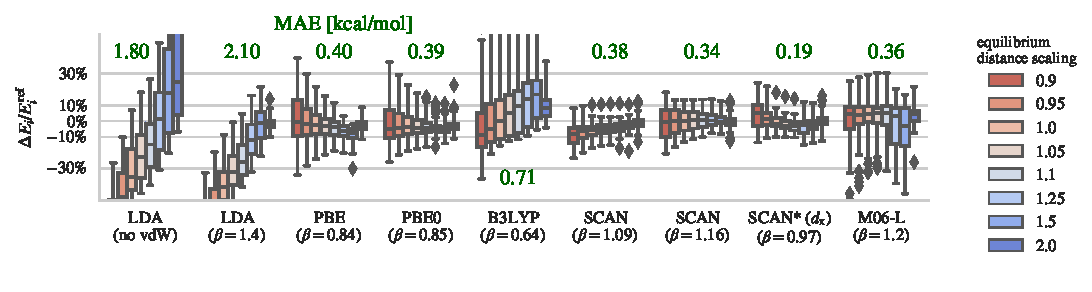
\includegraphics{../media/s66-dists}}
\caption{\textbf{Label.}
Text.
\label{fig:s66-dists}
}
\end{figure*}

\begin{figure*}
\makebox[\textwidth][c]{
\begin{tikzpicture}
\node [below right] at (0,0) {\bfseries a};
\node [below right] at (0,0) {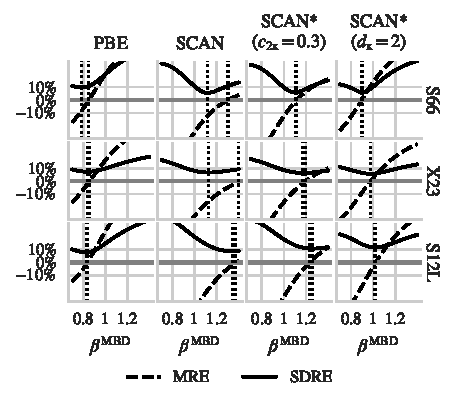
\includegraphics{../media/mbd-param-fitting.pdf}};
\node [below right] at (9.5,0) {\bfseries b};
\node [below right] at (9.5,0) {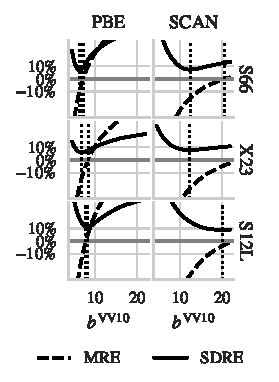
\includegraphics{../media/vv10-param-fitting.pdf}};
\node [below right] at (14.7,0) {\bfseries c};
\node [below right] at (14.7,0) {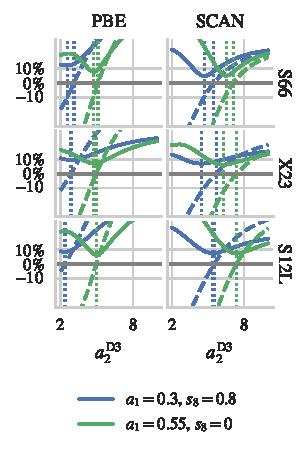
\includegraphics{../media/d3-param-fitting.pdf}};
\end{tikzpicture}
}
\caption{\textbf{Label.}
Text.
\label{fig:param-fitting}
}
\end{figure*}

\begin{figure}
\centering
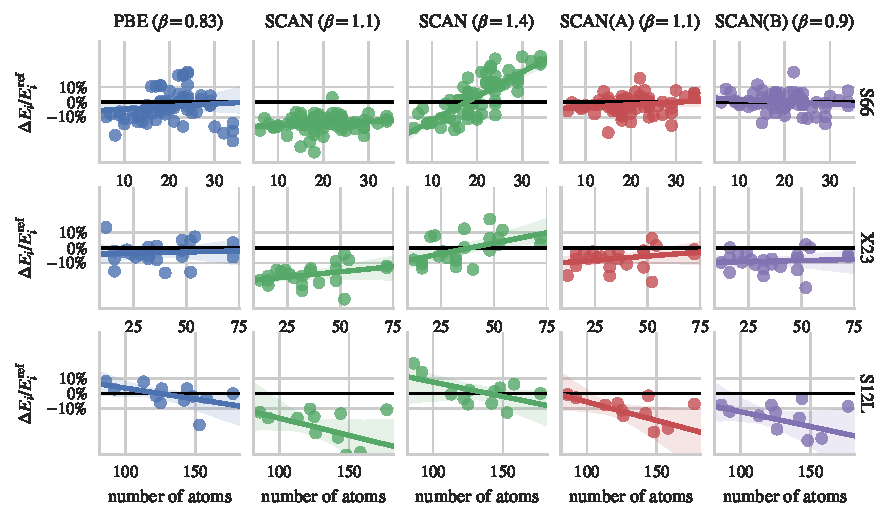
\includegraphics{../media/size-dependence}
\caption{\textbf{Label.}
Text.
\label{fig:size-dependence}
}
\end{figure}

\begin{figure}
\centering
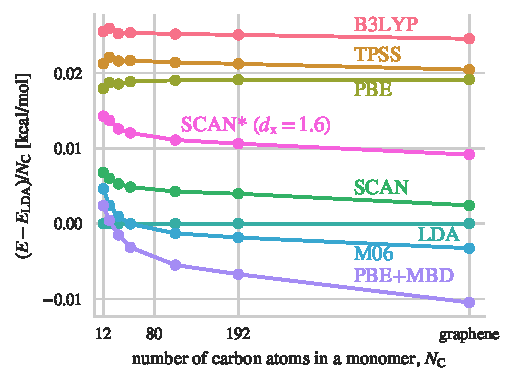
\includegraphics{../media/flakes}
\caption{\textbf{Label.}
Text.
\label{fig:flakes}
}
\end{figure}

\section{Conclusions}

